\documentclass[12pt]{article}
\usepackage[top=1in, bottom=1in, left=1in, right=1in]{geometry}

\usepackage{setspace}
\onehalfspacing

\usepackage{amssymb}
%% The amsthm package provides extended theorem environments
\usepackage{amsthm}
\usepackage{epsfig}
\usepackage{times}
\renewcommand{\ttdefault}{cmtt}
\usepackage{amsmath}
\usepackage{graphicx} % for graphics files
\usepackage{tabu}

% Draw figures yourself
\usepackage{tikz} 

% writing elements
%\usepackage{mhchem}

\usepackage{paralist}

% The float package HAS to load before hyperref
\usepackage{float} % for psuedocode formatting
\usepackage{xspace}

% from Denovo Methods Manual
\usepackage{mathrsfs}
\usepackage[mathcal]{euscript}
\usepackage{color}
\usepackage{array}

\usepackage[pdftex]{hyperref}
\usepackage[parfill]{parskip}

% math syntax
\newcommand{\nth}{n\ensuremath{^{\text{th}}} }
\newcommand{\ve}[1]{\ensuremath{\mathbf{#1}}}
\newcommand{\Macro}{\ensuremath{\Sigma}}
\newcommand{\rvec}{\ensuremath{\vec{r}}}
\newcommand{\vecr}{\ensuremath{\vec{r}}}
\newcommand{\omvec}{\ensuremath{\hat{\Omega}}}
\newcommand{\vOmega}{\ensuremath{\hat{\Omega}}}
\newcommand{\even}{\ensuremath{\phi^g}}
\newcommand{\odd}{\ensuremath{\vartheta^g}}
\newcommand{\evenp}{\ensuremath{\phi^{g'}}}
\newcommand{\oddp}{\ensuremath{\vartheta^{g'}}}
\newcommand{\Sn}{\ensuremath{S_N} }
\newcommand{\Ye}[2]{\ensuremath{Y^e_{#1}(\vOmega_#2)}}
\newcommand{\sigg}[1]{\ensuremath{\Macro^{g'\rightarrow g}_{s,#1}}}
\newcommand{\psig}{\ensuremath{\psi^g}}
%---------------------------------------------------------------------------
%---------------------------------------------------------------------------
\begin{document}
\begin{center}
{\bf NE 155/255, Fall 2019 \\
Equation Discretization\\
September 2019}
\end{center}

\setlength{\unitlength}{1in}
\begin{picture}(6,.1) 
\put(0,0) {\line(1,0){6.25}}         
\end{picture}

% We'll start from the general time-dependent NTE without delayed neutrons, with 7 
% independent variables. We need to discretize each variable.	

% \begin{align}
% &\frac{1}{v}\frac{\partial \psi}{\partial t}(\rvec,E,\omvec,t) + 
% \omvec\cdot  \nabla \psi(\rvec,E,\omvec,t)+
% \Sigma_t(\rvec,E)\psi(\rvec,E,\omvec,t)
% \\& \quad\quad\quad\quad =
% \int_0^{\infty}\int_{4\pi}
% \Sigma_s(\rvec, E'\rightarrow E,\omvec'\rightarrow\omvec)
% \psi(\rvec,E',\omvec',t)d\omvec'dE'\nonumber
% \\&\quad\quad\quad\quad\quad\quad +
% \frac{\chi_p(E)}{4\pi}\int_0^{\infty}\int_{4\pi}\nu(E')\Sigma_f(\rvec,E')
% \psi(\rvec,E',\omvec',t)d\omvec'dE'\nonumber
% \\&\quad\quad\quad\quad\quad\quad\quad\quad+S(\rvec, E, \omvec,t)\nonumber.
% \end{align}

% \section*{Time}

% Discretize the time interval $[0, T]$ into $N$ timesteps:

% \begin{figure}[h!]
%     \begin{center}
%     \includegraphics[keepaspectratio, width = 3.5 in]{time}
%     \end{center}
% \end{figure}

% Integrate the equation from $t=t_{n-1}$ to $t = t_n$, where we will use the 
% following definitions:

% \begin{align*}
% \psi(\vec{r}, E ,\vOmega, t_n) &= \psi_n(\vec{r}, E ,\vOmega)\\
% \Delta t &= t_{n} - t_{n-1}\\
% \bar{\psi}(\vec{r}, E ,\vOmega) &=
% \frac{1}{\Delta t} \int_{t_{n-1}}^{t_n} dt\: \psi(\vec{r}, E ,\vOmega, t)
% \end{align*}

% (Note: we're not specifying what actually happens in the integration; we're 
% generically defining a time-averaged angular flux).

% We also need to handle the time derivative term so that we can approximate it 
% on a time grid. We will use \textit{First Order Backward Difference} (more on 
% that later): 

% \[
% \frac{1}{v} \frac{\partial \psi}{\partial t}(\rvec,E,\omvec,t) =
% \frac{1}{v}\frac{\psi_n(\vec{r}, E ,\vOmega) - \psi_{n-1}(\vec{r}, E ,\vOmega)}
% {\Delta t}
% \]

% To get the time behavior of the solution, we integrate the entire transport 
% equation over each time step

% \[
% \int_{t_{n-1}}^{t_n} dt\: [\cdot]
% \]

% noting that

% \[
% \int_{t_{n-1}}^{t_n} dt\: \bigl(\frac{1}{v}\frac{\psi_n(\vec{r}, E ,\vOmega) - 
% \psi_{n-1}(\vec{r}, E ,\vOmega)}{\Delta t}\bigr) =
% \frac{1}{v}\frac{\psi_n(\vec{r}, E ,\vOmega) - \psi_{n-1}(\vec{r}, E ,\vOmega)}
% {\Delta t}
% \]

% which gives

% \begin{align*}
% \frac{1}{v}&
% \frac{\psi_n(\vec{r}, E ,\vOmega)-\psi_{n-1}(\vec{r}, E ,\vOmega)}{\Delta t} 
% + \omvec\cdot  \nabla  \bar{\psi}(\vec{r}, E ,\vOmega) 
% + \Sigma_t(\rvec,E)\bar{\psi}(\vec{r}, E ,\vOmega) 
% = \\& \int_0^{\infty}dE'\int_{4\pi}d\omvec'\:
% \Sigma_s(\rvec, E'\rightarrow E,\omvec'\rightarrow\omvec)
% \bar{\psi}(\vec{r}, E' ,\vOmega')
% \\&+ \frac{\chi_p(E)}{4\pi}\int_0^{\infty}dE'\:
% \nu(E')\Sigma_f(\rvec,E')\int_{4\pi}d\omvec'\:
% \bar{\psi}(\vec{r}, E' ,\vOmega')
% +\bar{S}(\rvec, E, \omvec)
% \end{align*}

% Note(!): we now have two unknowns ($\psi_n$ and $\bar{\psi}$). We need to 
% relate them; we choose a linear combination with a weighting parameter $\beta$:

% \[
% \bar{\psi} = \beta \psi_n + (1 - \beta)\psi_{n-1}
% \]

% We substitute this in to get

% \begin{align*}
% \omvec\cdot  \nabla  \bar{\psi}(\vec{r}, E ,\vOmega) 
% &+ \bigl(\Sigma_t + \frac{1}{v \beta \Delta t}\bigr)
% \bar{\psi}(\vec{r}, E ,\vOmega) 
% =  \frac{1}{v \beta \Delta t} \psi_{n-1}(\vec{r}, E ,\vOmega) \\
% &+ \int_0^{\infty}dE'\int_{4\pi}d\omvec'\:
% \Sigma_s(\rvec, E'\rightarrow E,\omvec'\rightarrow\omvec)
% \bar{\psi}(\vec{r}, E' ,\vOmega')
% \\&+ \frac{\chi_p(E)}{4\pi}\int_0^{\infty}dE'\:
% \nu(E')\Sigma_f(\rvec,E')\int_{4\pi}d\omvec'\:
% \bar{\psi}(\vec{r}, E' ,\vOmega')
% +\bar{S}(\rvec, E, \omvec)
% \end{align*}

% We solve this for $n=1, \dots, N$ and $\psi_0$ is given (initial value 
% problem!).

%---------------------------------------------------------------------------
% \subsubsection*{Aside about Finite Difference}

% Finite difference is a common way to numerically approximate derivatives. 
% \textbf{Example} Given $f$ is $ C^2 \in [a,b]$ and $x_0 \in [a,b]$, find an 
% approximation to $f'(x_0)$ and or $f''(x_0)$, etc.

% We're going to come at this from \textbf{Taylor's theorem}, which gives an approximation of a k-times differentiable function around a given point by a k-th order Taylor polynomial.

% \[
% f(x) = \sum_{0}^{k} \frac{f^{(n)}(x_0)}{n!}(x - x_0)^n
% \]
% % https://en.wikipedia.org/wiki/Taylor%27s_theorem

% To approximate any type of derivative to a specified order of accuracy, we 
% Taylor expand several points in our collection. Then, we choose how many 
% points to combine and in what ways. 

% \begin{align*}
% f(x_0) &= f(x_0)\\
% f(x_0 \pm h) &= f(x_0) \pm hf'(x_0) + h^2\frac{f''(x_0)}{2} \pm 
% h^3\frac{f'''(x_0)}{6} + f^{(4)}(c_1)\frac{h^4}{24} \\
% f(x_0 \pm 2h) &= f(x_0) \pm 2h f'(x_0) + 2 h^2 f''(x_0) \pm
% \frac{4}{3} h^3 f'''(x_0) + \frac{2}{3}h^4 f^{(4)}(c_2)
% \end{align*}

% We combine the expanded expressions, rearrange to group terms, and solve for 
% what we're interested in:

% For \underline{$O(h)$ Backwards Difference}: combine the point and the next 
% point backward:

% \begin{align*}
% f(x_0) &= f(x_0)\\
% f(x_0 - h) &= f(x_0) - hf'(x_0) + h^2\frac{f''(c)}{2}\\
% a f(x_0) &+ b f(x_0 - h) = f'(x_0) \\
% a f(x_0) &+ b \bigl(f(x_0) - hf'(x_0) + h^2\frac{f''(c)}{2} \bigr) = f'(x_0) \\
% (a+b)f(x_0) &-bh f'(x_0) + b h^2\frac{f''(c)}{2} = f'(x_0)
% \end{align*}

% Now, we solve for the coefficients to get what we want

% \begin{align*}
% a+b = 0 &\quad -bh = 1 \\
% b &= -\frac{1}{h} \quad a = \frac{1}{h}
% \end{align*}


% We now sub in $a$ and $b$. This gives the first order ($O(h)$) Backwards 
% Difference approximation, which is what we used for the time derivative.

% \begin{align*}
% \text{error }&= -\frac{1}{h}h^2\frac{f''(c)}{2}\\
% f'(x_0) &= \frac{f(x_0) - f(x_0 - h)}{h} + \frac{1}{2}hf''(\mu)
% \end{align*}

% A note about what points to choose: you want to think about how your equations 
% transmit information. A perturbation of the initial (or boundary) data of an 
% \textit{elliptic or parabolic} equation is felt at once by essentially all 
% points in the domain.The solutions of hyperbolic equations are ``wave-like.''
% If a disturbance is made in the initial data of a hyperbolic differential 
% equation, then not every point of space feels the disturbance at once.

We'll start from the general time-independent NTE without delayed neutrons, with 6 
independent variables. We need to discretize each variable. 

\begin{align}
&\omvec\cdot  \nabla \psi(\rvec,E,\omvec)+
\Sigma_t(\rvec,E)\psi(\rvec,E,\omvec) \nonumber
\\&
\quad\quad\quad\quad =
\int_0^{\infty}\int_{4\pi}
\Sigma_s(\rvec, E'\rightarrow E,\omvec'\rightarrow\omvec)
\psi(\rvec,E',\omvec')d\omvec'dE'
\\&\quad\quad\quad\quad\quad\quad +
\frac{\chi_p(E)}{4\pi}\int_0^{\infty}\int_{4\pi}\nu(E')\Sigma_f(\rvec,E')
\psi(\rvec,E',\omvec')d\omvec'dE'\nonumber
\\&\quad\quad\quad\quad\quad\quad\quad\quad+S(\rvec, E, \omvec)\nonumber
\end{align}

%---------------------------------------------------------------------------
%---------------------------------------------------------------------------
\section*{Energy Discretization}

We'll handle the energy dimension by breaking continuous energy 
into $G$ groups, where group $g$ is [$E_{g}, E_{g-1}$]:

\begin{center}
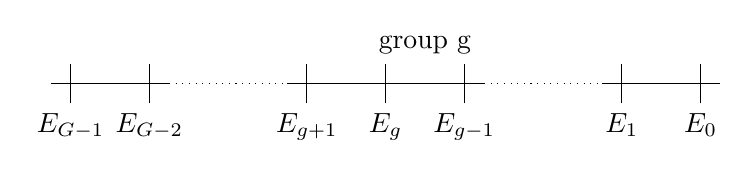
\begin{tikzpicture}
\draw (-.25,0)--(1.25,0);
\draw[dotted] (1.25,0)--(2.75,0);
\draw (2.75,0)--(5.25,0);
\draw[dotted] (5.25,0)--(6.75,0);
\draw (6.75,0)--(8.25,0);
%\draw (4,0)--(5.25,0);
\draw (0,-.25)--(0,.25);
\draw (1,-.25)--(1,.25);
%\draw (2,-.25)--(2,.25);
\draw (3,-.25)--(3,.25);
\draw (4,-.25)--(4,.25);
\draw (5,-.25)--(5,.25);
\draw (7,-.25)--(7,.25);
\draw (8,-.25)--(8,.25);
\node[below] at (0,-.25) {$E_{G-1}$};
\node[below] at (1,-.25) {$E_{G-2}$};
\node[below] at (3,-.25) {$E_{g+1}$};
\node[below] at (4,-.25) {$E_g$};
\node[above] at (4.5, .25) {group g};
\node[below] at (5,-.25) {$E_{g-1}$};
\node[below] at (7,-.25) {$E_{1}$};
\node[below] at (8,-.25) {$E_0$};
\end{tikzpicture}
\end{center}

We will solve for group-integrated values in each energy bin using the following definitions:

\begin{align*}
\psi_g(\rvec, \vOmega) &\equiv \int_{E_g}^{E_{g-1}} dE\:
\psi(\rvec, \vOmega, E) \qquad
\phi_g(\rvec) \equiv \int_{E_g}^{E_{g-1}} dE\: \phi(\rvec,  E)\\
S_g(\rvec, \vOmega) &\equiv \int_{E_g}^{E_{g-1}} dE\:
S(\rvec, \vOmega, E) \qquad
\chi_g \equiv \int_{E_g}^{E_{g-1}} dE\: \chi(E)
\end{align*}

To perform these integrals, we need to introduce approximations. We
\textit{assume that each item is separable in energy}.

For example:

\[
\psi(\vec{r}, \vOmega, E) \approx f(E)\psi_g(\vec{r}, \vOmega)\:,
\quad E_g < E \leq E_{g-1}\:,
\]

where $f(E)$ is normalized such that $\int_g dE\: f(E) = 1$.

Next, we need a way to create multigroup cross sections. Options for how to do 
that in more detail are covered in NE 250. Here we will do the most
common/generic approach: weight with the angular flux:

\[
\Sigma_{t,g}(\vec{r}) \equiv \frac{\int_{E_g}^{E_{g-1}} dE\:
\Sigma_t(\rvec, E) f(E)}{\int_{E_g}^{E_{g-1}} dE\: f(E)} =
\frac{\int_{E_g}^{E_{g-1}} dE\:
\Sigma_t(\rvec, E) \psi(\rvec, \vOmega, E)}{\int_{E_g}^{E_{g-1}} dE\:
\psi(\rvec, \vOmega, E)}
\]

We do the same thing for fission (not shown here). Scattering requires an 
extra integral:

\begin{align*}
\Sigma_{s}^{g'\rightarrow g}(\vecr, \vOmega' \cdot \vOmega) & \equiv 
\frac{\int_{E_g}^{E_{g-1}} dE \int_{E_{g'}}^{E_{g'-1}} dE' \:
\Sigma_s(\vecr,E'\rightarrow E, \vOmega' \cdot \vOmega) f(E')}
{\int_{E_{g'}}^{E_{g'-1}} dE' \: f(E')}\\
& \equiv \frac{\int_{E_g}^{E_{g-1}} dE \int_{E_{g'}}^{E_{g'-1}} dE' \:
\Sigma_s(\vecr, E'\rightarrow E, \vOmega' \cdot \vOmega)
\psi(\rvec, \vOmega', E')}{\int_{E_{g'}}^{E_{g'-1}} dE' \:
\psi(\rvec, \vOmega', E')}
\end{align*}

Using these definitions, we can write a transport equation for each 
group, $g = 0,\dots, G-1$:

\begin{align*}
[\vOmega \cdot \nabla + \Sigma_{t,g}(\vec{r})]\psi_g(\vec{r}, \vOmega) =  
\sum_{g'=0}^{G-1} \int_{4 \pi} d\vOmega'\:
&\Sigma_{s}^{g'\rightarrow g}(\vec{r}, \vOmega' \cdot \vOmega) \psi_{g'}(\vec{r}, \vOmega')\\
&+\frac{\chi_g}{4 \pi}\sum_{g'=0}^{G-1} \nu_{g'}\Sigma_{f,g'}(\vec{r})
\phi_{g'}(\vec{r}) + S_g(\vec{r}, \vOmega),
\end{align*}

giving $G$ coupled equations. Note that the coupling may cause iteration 
because of the exchange of particles between energy groups (upscattering!). 

These equations are \textbf{exact} in the unique case where (1) the 
separability in energy holds and (2) the cross sections are constant within 
each energy group. 

\end{document}
